% Archivo principal de compilación.
% El contenido del reporte está en main.tex.
\documentclass[12pt,oneside]{template/liverpoolthesis}
% !TEX root = ../Actividad2_Espino_Heriberto.tex
% Select the discipline once; the template chooses a suitable bibliography
% style. General or unknown disciplines fall back to APA. An explicit
% style=... option can override the automatic choice when required.
\usepackage[discipline=computer-science]{template/liverpoolthesis}
\usepackage[utf8]{inputenc}
\usepackage[T1]{fontenc}
\usepackage[spanish,es-nodecimaldot]{babel}

\makeatletter
% Sobreescritura del autómata lingüístico de babel.
\addto\captionsspanish{%
  \renewcommand{\chaptername}{Ejercicio}%
  \renewcommand{\appendixname}{Anexo}%
}
\makeatother

% Controls whether heading numbers are printed.
\setcounter{secnumdepth}{2}
\graphicspath{{figuras/}}



\begin{document}

% ---------- Datos de la portada ----------
\title{Actividad 2: Componentes de una computadora y procesos}
\author{Heriberto Espino Montelongo \\
  ID: 175199\\[1em]
  \text{Profesor:} Dr. Victor Giovanni Morales Murillo}
\faculty{Universidad de las Américas Puebla (UDLAP)}
\school{Licenciatura en Ciencia de Datos}
\degree{Curso: Programación Concurrente}
\date{Fecha de entrega: 20 de agosto de 2026}
\subject{Análisis de los componentes de una computadora e implementación de procesos}

\frontmatter
\maketitle
\mainmatter
\listoffigures

\begin{abbreviations}
  \item[OS] \textit{Operating System}: sistema operativo que administra los recursos de hardware.
  \item[CPU] \textit{Central Processing Unit}: procesador que controla la computadora.
  \item[RAM] \textit{Random Access Memory}: memoria principal que mantiene temporalmente instrucciones y datos.
  \item[I/O] \textit{Input/Output}: entrada y salida de datos.
  \item[PC] \textit{Program Counter}: contiene la dirección de la siguiente instrucción.
  \item[IR] \textit{Instruction Register}: contiene la instrucción que está siendo ejecutada.
  \item[MAR] \textit{Memory Address Register}: especifica la dirección de memoria que será leída o escrita.
  \item[MBR] \textit{Memory Buffer Register}: contiene los datos que se escriben o leen de la memoria.
  \item[I/O AR] \textit{Input/Output Address Register}: especifica el dispositivo de I/O.
  \item[I/O BR] \textit{Input/Output Buffer Register}: intercambia datos con un I/O module.
  \item[AC] \textit{Accumulator}: register utilizado como almacenamiento temporal.
  \item[CISC] \textit{Complex Instruction Set Computer}: arquitectura de procesador con un conjunto de instrucciones complejas e integradas.
  \item[RISC] \textit{Reduced Instruction Set Computer}: arquitectura de procesador simplificada orientada a la ejecución rápida de instrucciones básicas.
  \item[x86] Arquitectura de juego de instrucciones CISC desarrollada originalmente por Intel para procesadores de 32 y 64 bits (x86\_64).
  \item[ARM] \textit{Advanced RISC Machine}: arquitectura de procesamiento basada en diseño RISC de alto rendimiento y bajo consumo energético.
  \item[PID] \textit{Process Identifier}: identificador único asignado por el kernel a un proceso en ejecución.
  \item[PPID] \textit{Parent Process Identifier}: identificador de proceso correspondiente al proceso padre que generó la ejecución actual.
  \item[UID] \textit{User Identifier}: número entero que identifica de forma persistente al usuario propietario del proceso.
  \item[EUID] \textit{Effective User Identifier}: identificador de usuario efectivo que el sistema evalúa para otorgar permisos y accesos en tiempo de ejecución.
\end{abbreviations}


\chapter{Funcionamiento de una Computadora}

Explica lo más claro posible el funcionamiento de cada componente de una
computadora con base en la lectura del punto anterior, centrándose en el tema 1.3
instruction execution.

\section{Componentes de una computadora e Instruction Execution}

En general, una computadora tiene cuatro componentes principales: el procesador
procesa los datos, la \textit{main memory} mantiene las instrucciones y los
datos, los \textit{I/O modules} los mueven entre la computadora y los
dispositivos externos, y el \textit{System Bus} permite la comunicación entre
el CPU, la main memory y los I/O modules.

\begin{figure}[H]
    \centering
    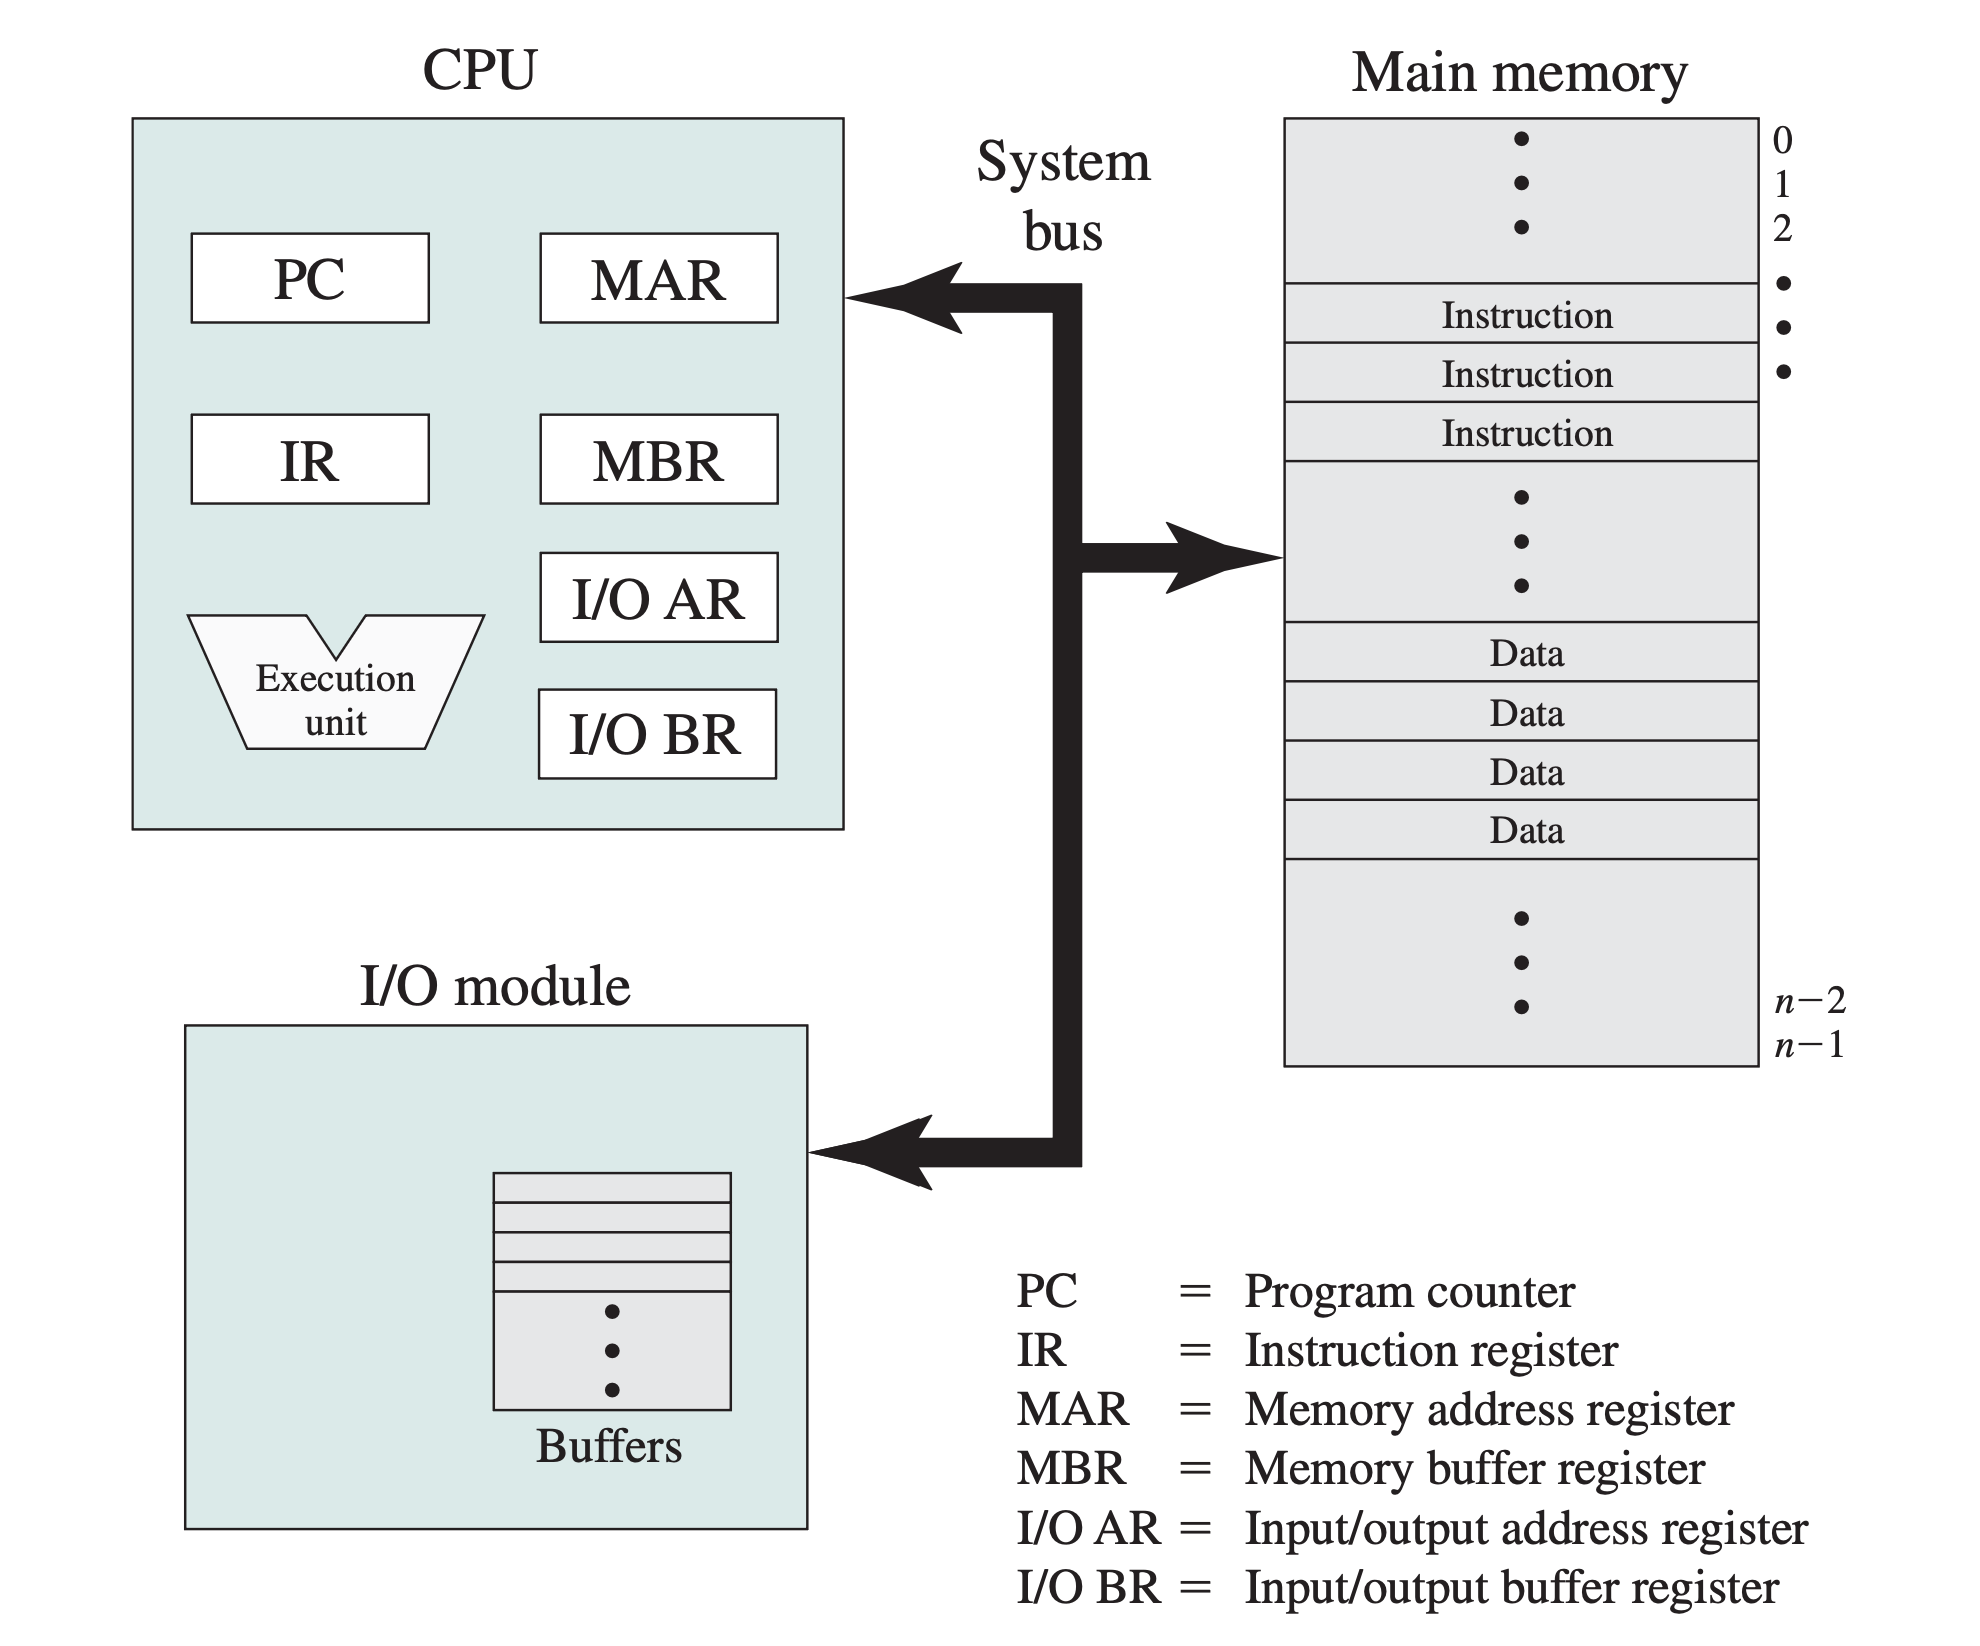
\includegraphics[width=0.66\textwidth]{3.png}
    \caption{Componentes principales de una computadora y su comunicación
    mediante el System Bus.}
    \label{fig:componentes}
\end{figure}


\subsection{CPU y registers}

El \textit{Central Processing Unit} (CPU) es el procesador que controla la
operación de la computadora. Dentro del CPU existen los
\textit{registers}, que guardan  instrucciones, direcciones o
datos que se necesitan en ese momento.

El \textit{Program Counter} (PC) contiene la dirección de la siguiente
instrucción de la que se realizará el \textit{fetch}. El
\textit{Instruction Register} (IR) contiene la instrucción que se está
ejecutando, mientras que la \textit{Execution Unit} realiza la operación
indicada por esa instrucción.

El \textit{Memory Address Register} (MAR) especifica qué dirección de memoria
será la siguiente en ser leída o escrita. El \textit{Memory Buffer Register}
(MBR) contiene los datos que se escribirán en la memoria o recibe los datos
que se leen de ella.

Para las operaciones de I/O, el \textit{I/O Address Register} (I/O AR)
especifica con cuál dispositivo se realizará la operación, mientras que el
\textit{I/O Buffer Register} (I/O BR) se utiliza para intercambiar datos entre
el procesador y un I/O module.

\subsection{Main Memory}

La \textit{main memory}, también llamada
\textit{Random Access Memory} (RAM), guarda temporalmente las instrucciones y
los datos que necesita el procesador. Es una memoria \textit{volatil}, por lo que su
contenido desaparece cuando la computadora se apaga. En cambio, la memoria
secundaria, como un disco o SSD, conserva los datos.

También existe una \textit{memory hierarchy}. Los registers están dentro del
CPU y mantienen los valores que se necesitan inmediatamente. Después se
encuentran las memorias caché L1, L2 y L3, que normalmente están integradas en
el chip del procesador. Luego está la RAM y finalmente la memoria secundaria,
como un SSD.

\subsection{I/O Modules}

Los I/O devices son los dispositivos físicos, como un disco, un SSD, un
teclado, un mouse o unos audífonos.
El I/O module es el componente intermediario que permite que esos dispositivos
se comuniquen con el procesador y la main memory. Por ejemplo, el teclado y el
mouse entregan datos de entrada, los audífonos reciben datos de salida y un
disco o SSD puede leer y escribir datos.

El \textit{buffer} es un espacio temporal que
mantiene temporalmente bloques de datos y \textit{amortigua} la diferencia de
velocidad entre dispositivos, mientras esperan ser enviados, recibidos o procesados. Esto evita que cada
componente tenga que esperar y transferir los datos uno por uno.

\subsection{Programa e Instruction Cycle}

\textbf{Programa:} es un \textit{set de instrucciones} guardadas en memoria
que el procesador obtiene mediante \textit{fetch} y después ejecuta.

El procesamiento de una instrucción tiene dos etapas:

\begin{enumerate}
    \item \textbf{Fetch stage:} el procesador realiza el fetch de la siguiente
    instrucción desde la memoria. El PC contiene su dirección y la instrucción
    obtenida se coloca en el IR.

    \item \textbf{Execute stage:} el procesador interpreta la instrucción y la
    Execution Unit realiza la operación indicada.
\end{enumerate}

Al procesamiento completo de una instrucción se le llama
\textit{Instruction Cycle}. El procesador repite el fetch stage y el execute
stage porque un programa contiene varias instrucciones que deben ejecutarse.

\begin{figure}[H]
    \centering
    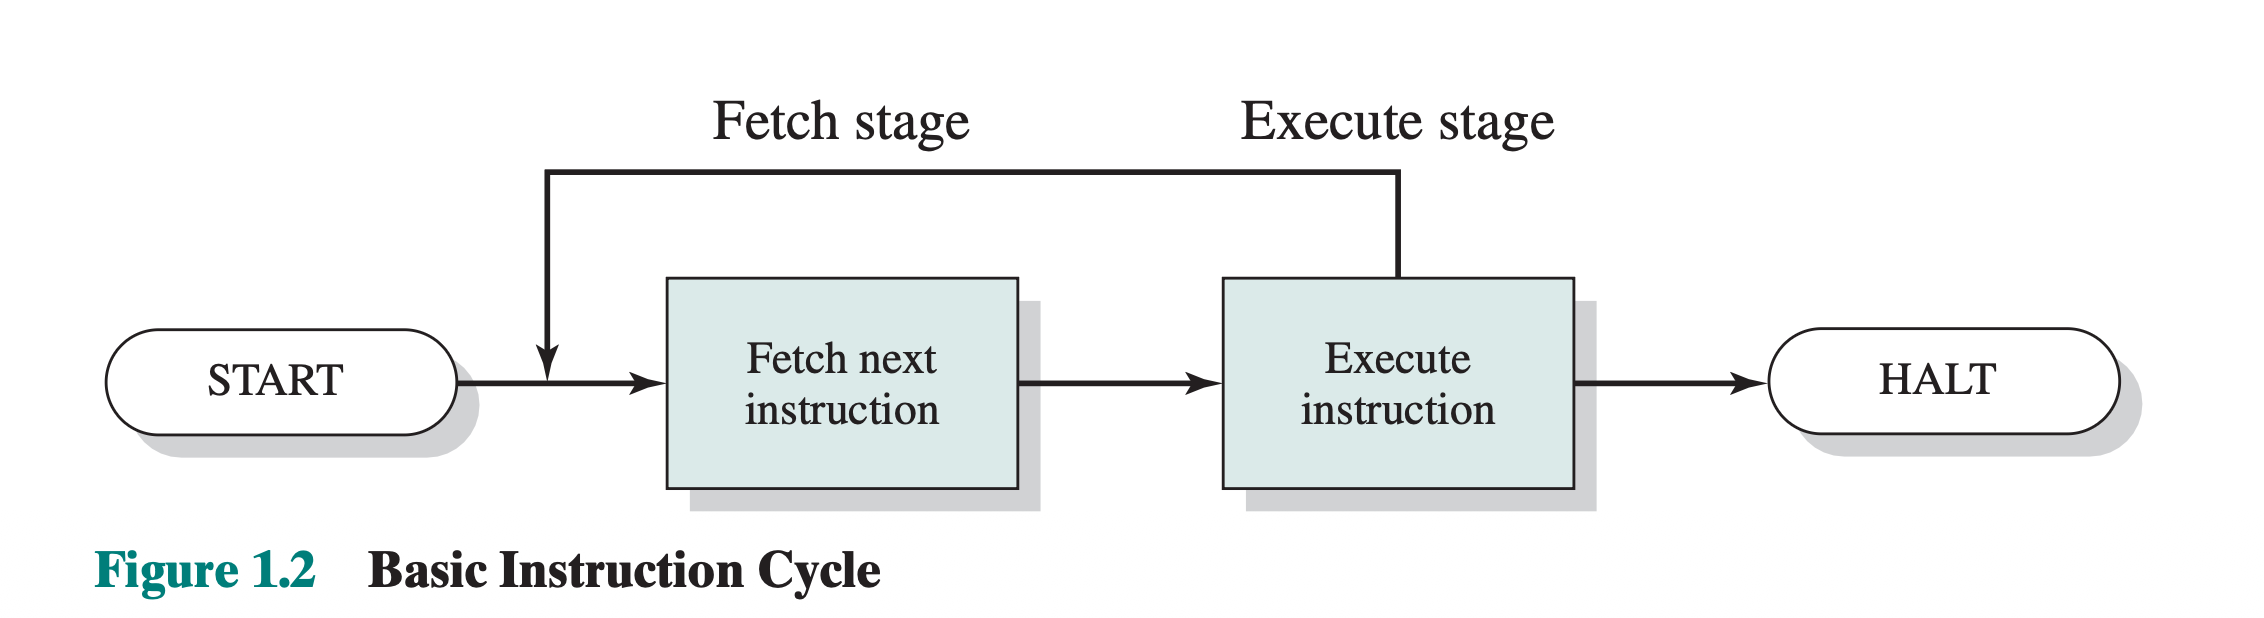
\includegraphics[width=0.88\textwidth]{2.png}
    \caption{Basic Instruction Cycle.}
    \label{fig:instruction-cycle}
\end{figure}

La Figura~\ref{fig:instruction-cycle} resume este proceso. Después de cada
fetch, el PC aumenta para apuntar a la siguiente dirección de
memoria. El proceso termina cuando se encuentra una instrucción de \textit{HALT},
(o cuando se apaga el procesador o cuando ocurre un error).


\subsection{Formato de una instrucción}

En la Figura 1.3, cada instrucción tiene
16 bits. Los primeros 4 bits (que esta formado por una letra en formato hexadecimal) forman el \textit{opcode}, que indica la operación
que realizará el procesador, y los 12 bits restantes forman el
\textit{address}, que indica una dirección de memoria.

\begin{figure}[H]
    \centering
    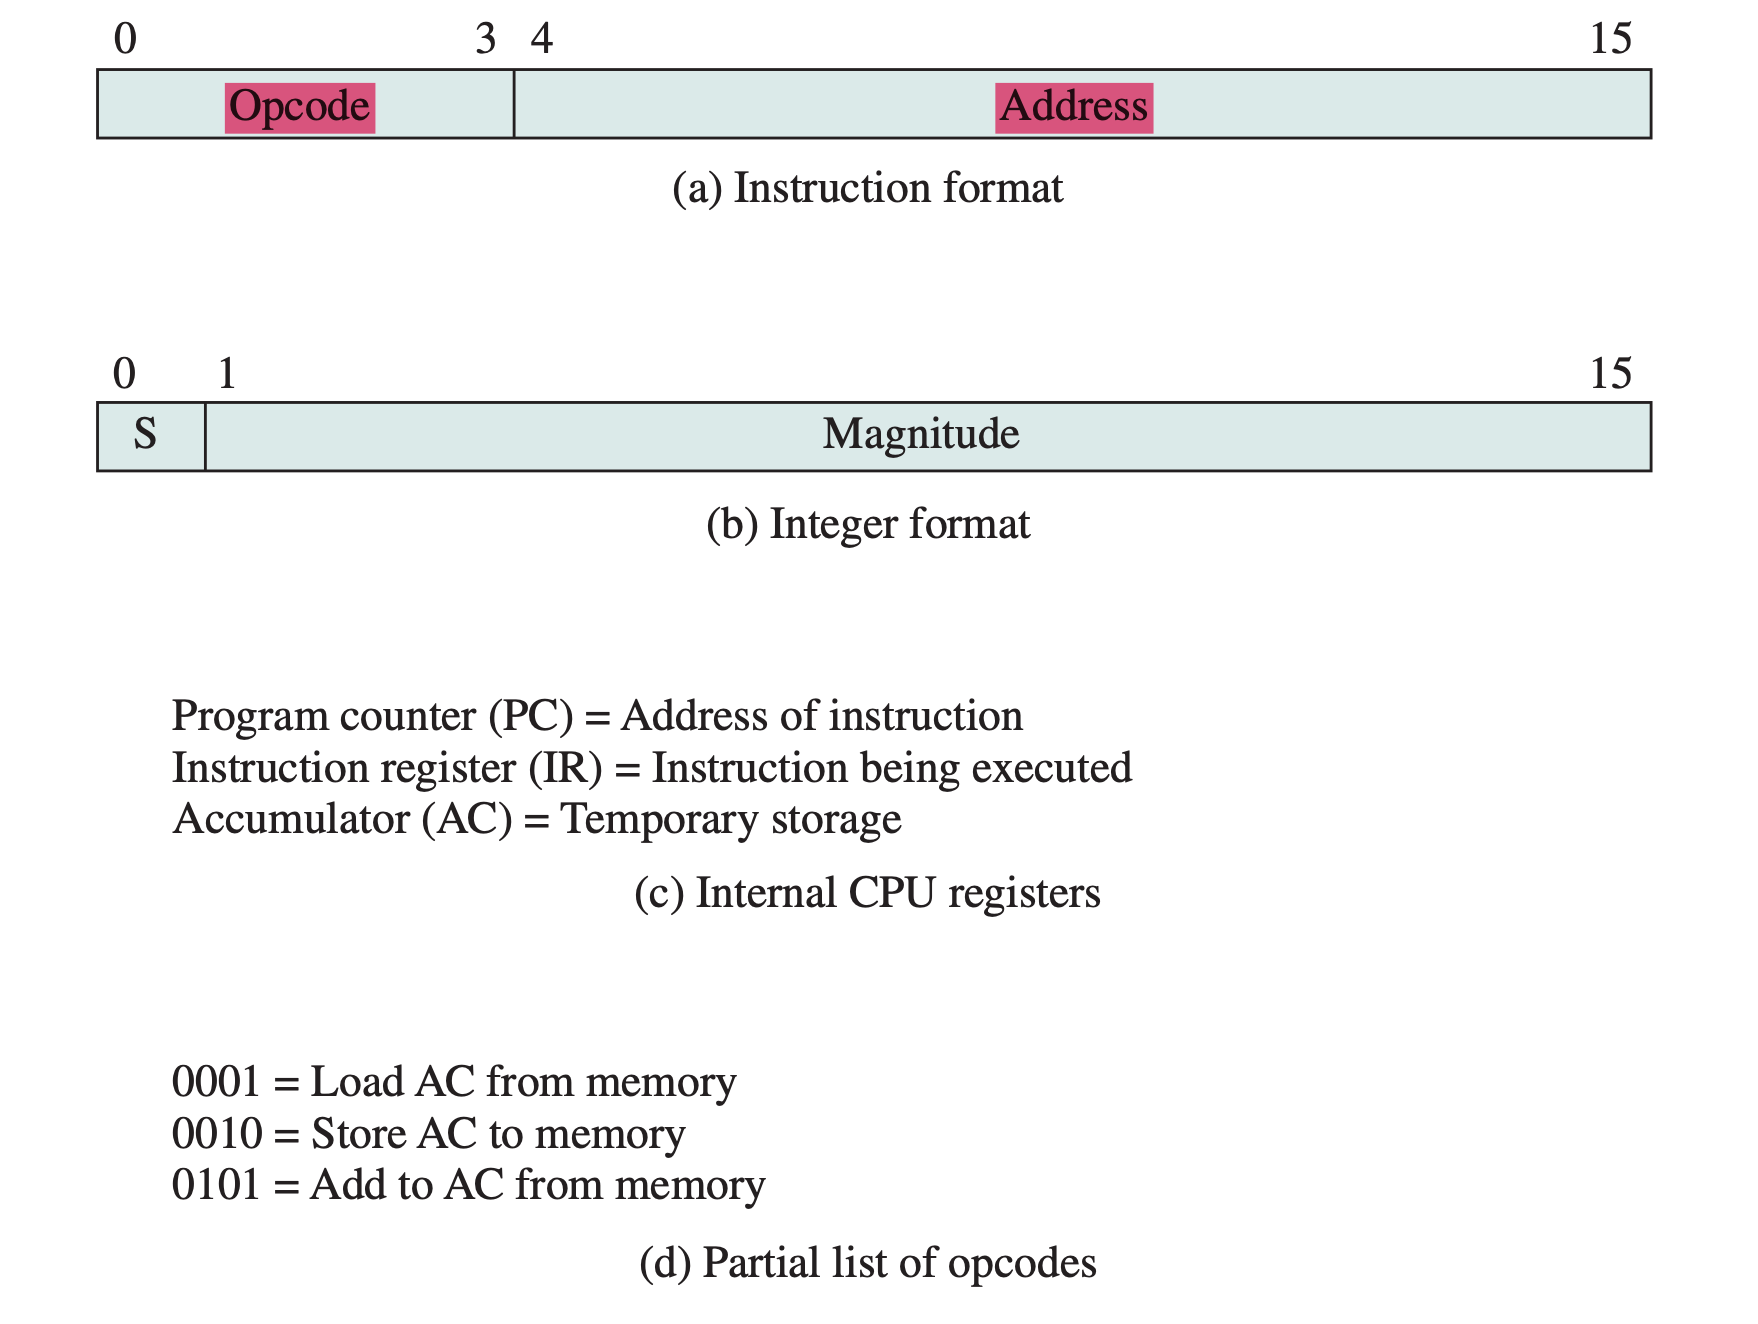
\includegraphics[width=0.73\textwidth]{1.png}
    \caption{Formato de instrucciones y registers de una máquina hipotética.}
    \label{fig:instruction-format}
\end{figure}

\subsection{Instrucciones}
La ejecución de una instrucción puede producir cuatro tipos generales de
acciones:

\begin{itemize}
    \item \textbf{Processor-memory:} se transfieren datos entre el procesador y la memoria.

    \item \textbf{Processor-I/O:} se transfieren datos entre el procesador y un I/O device.

    \item \textbf{Data processing:} el procesador realiza una operación.

    \item \textbf{Control:} una instrucción modifica la secuencia de ejecución del PC.
\end{itemize}

\subsection{Ejecución de un programa mediante los componentes de la computadora}

Antes de ejecutar un programa, este se encuentra almacenado en la memoria
secundaria. El OS carga en
la main memory las instrucciones y los datos necesarios desde el dispositivo de almacenamiento, a través de
un \textit{I/O module} y sus buffers, utilizando el \textit{System Bus}.

Una vez que las instrucciones están cargadas, el CPU comienza
el \textit{Instruction Cycle}. Este proceso ocurre de la siguiente manera:

\begin{enumerate}
    \item El PC contiene la dirección de la siguiente
    instrucción de la que se realizará el fetch.

    \item La dirección se coloca en el MAR,
    que especifica la ubicación de memoria que debe leerse.

    \item La main memory entrega la instrucción. Esta pasa por el
    MBR y después se coloca en el
    IR.

    \item El PC normalmente aumenta para apuntar a la siguiente instrucción
    guardada en memoria.

    \item El CPU interpreta la instrucción que se encuentra en el IR con el 
    \textit{opcode}, que indica qué operación debe realizarse, y un
    \textit{address}, que señala una dirección de memoria.

    \item La \textit{Execution Unit} ejecuta la operación indicada por el
    opcode. 

    \item El resultado puede mantenerse temporalmente en un register, guardarse
    en la main memory o enviarse a un I/O device.

    \item El CPU vuelve a realizar el fetch de la siguiente instrucción y
    repite el Instruction Cycle.
\end{enumerate}

La memoria secundaria conserva el programa, los I/O modules permiten
transferirlo, los buffers mantienen temporalmente los datos, el System Bus
comunica los componentes, la RAM mantiene las instrucciones y los datos que
se están utilizando, y el CPU realiza repetidamente los fetch stages y execute
stages hasta encontrar una instrucción de \textit{HALT}.


\chapter{Instrucciones e Identificadores en C}

Ejecuta el siguiente código fuente en C en una máquina virtual de Linux y agrega
la captura de pantalla de la ejecución.

\begin{figure}[H]
    \centering
    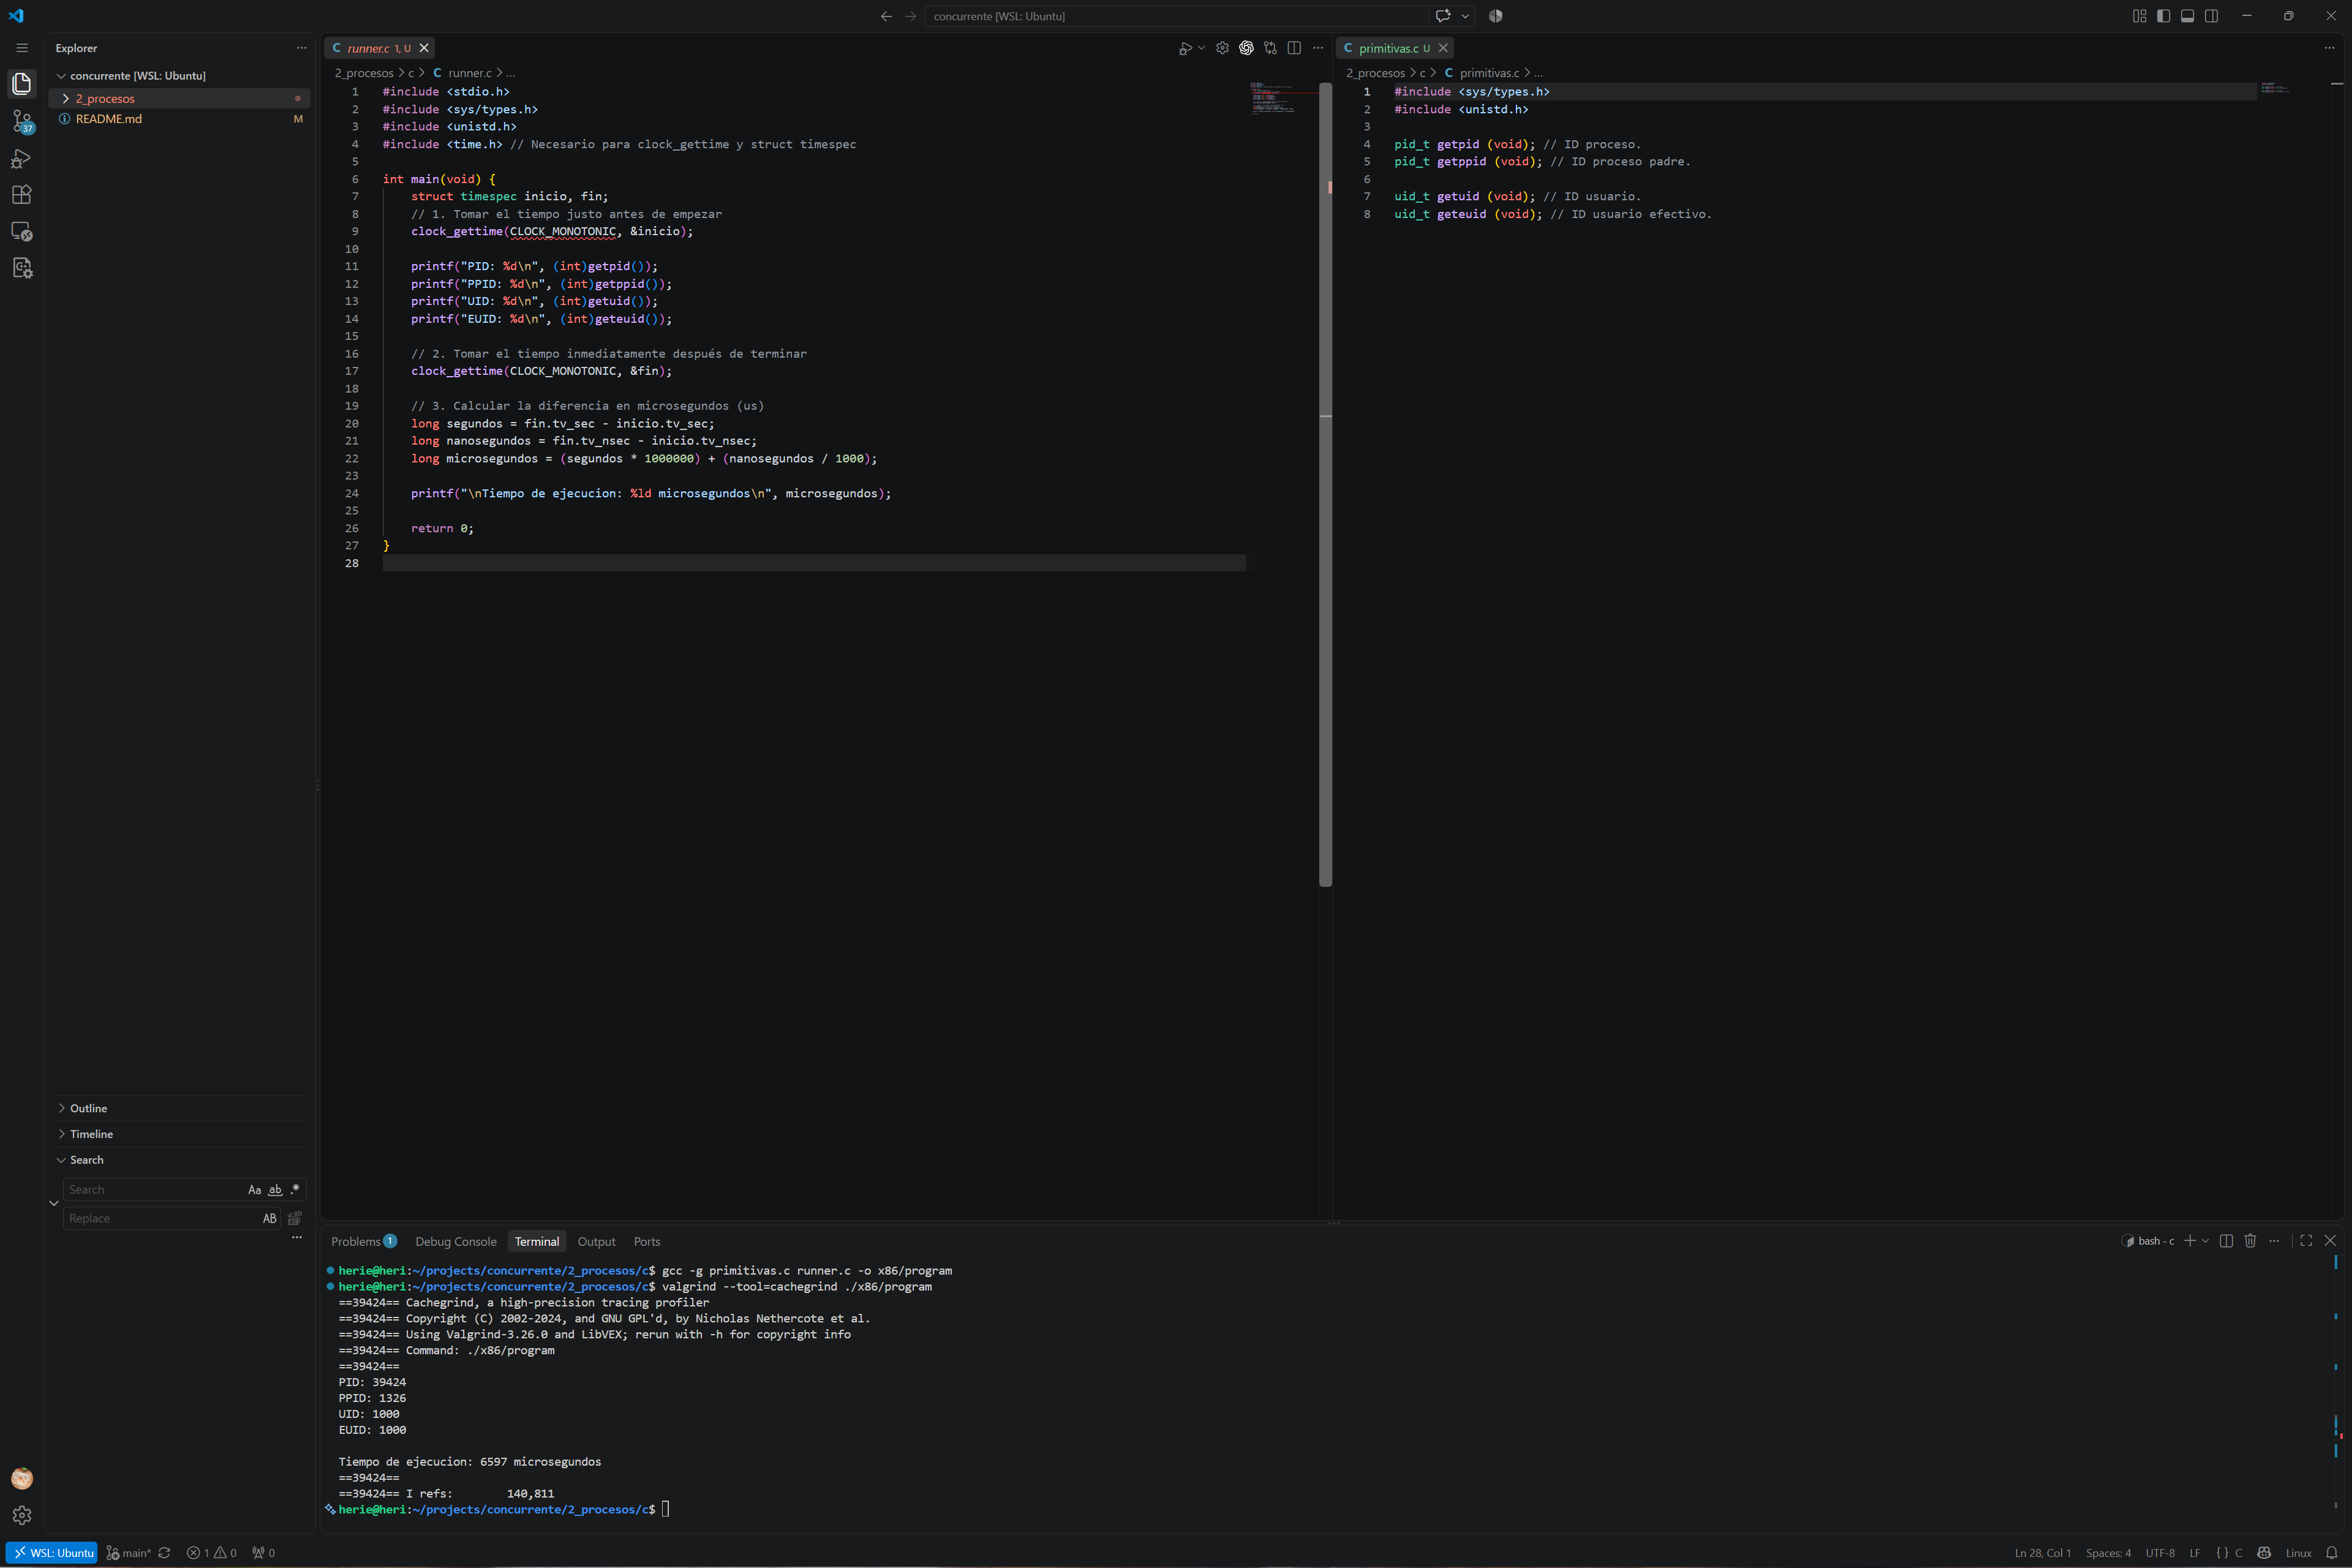
\includegraphics[width=0.73\textwidth]{4.png}
    \caption{Ejercicio 2 ejecutado en WSL en un procesador x86}
    \label{fig:execution-wsl}
\end{figure}

\begin{figure}[H]
    \centering
    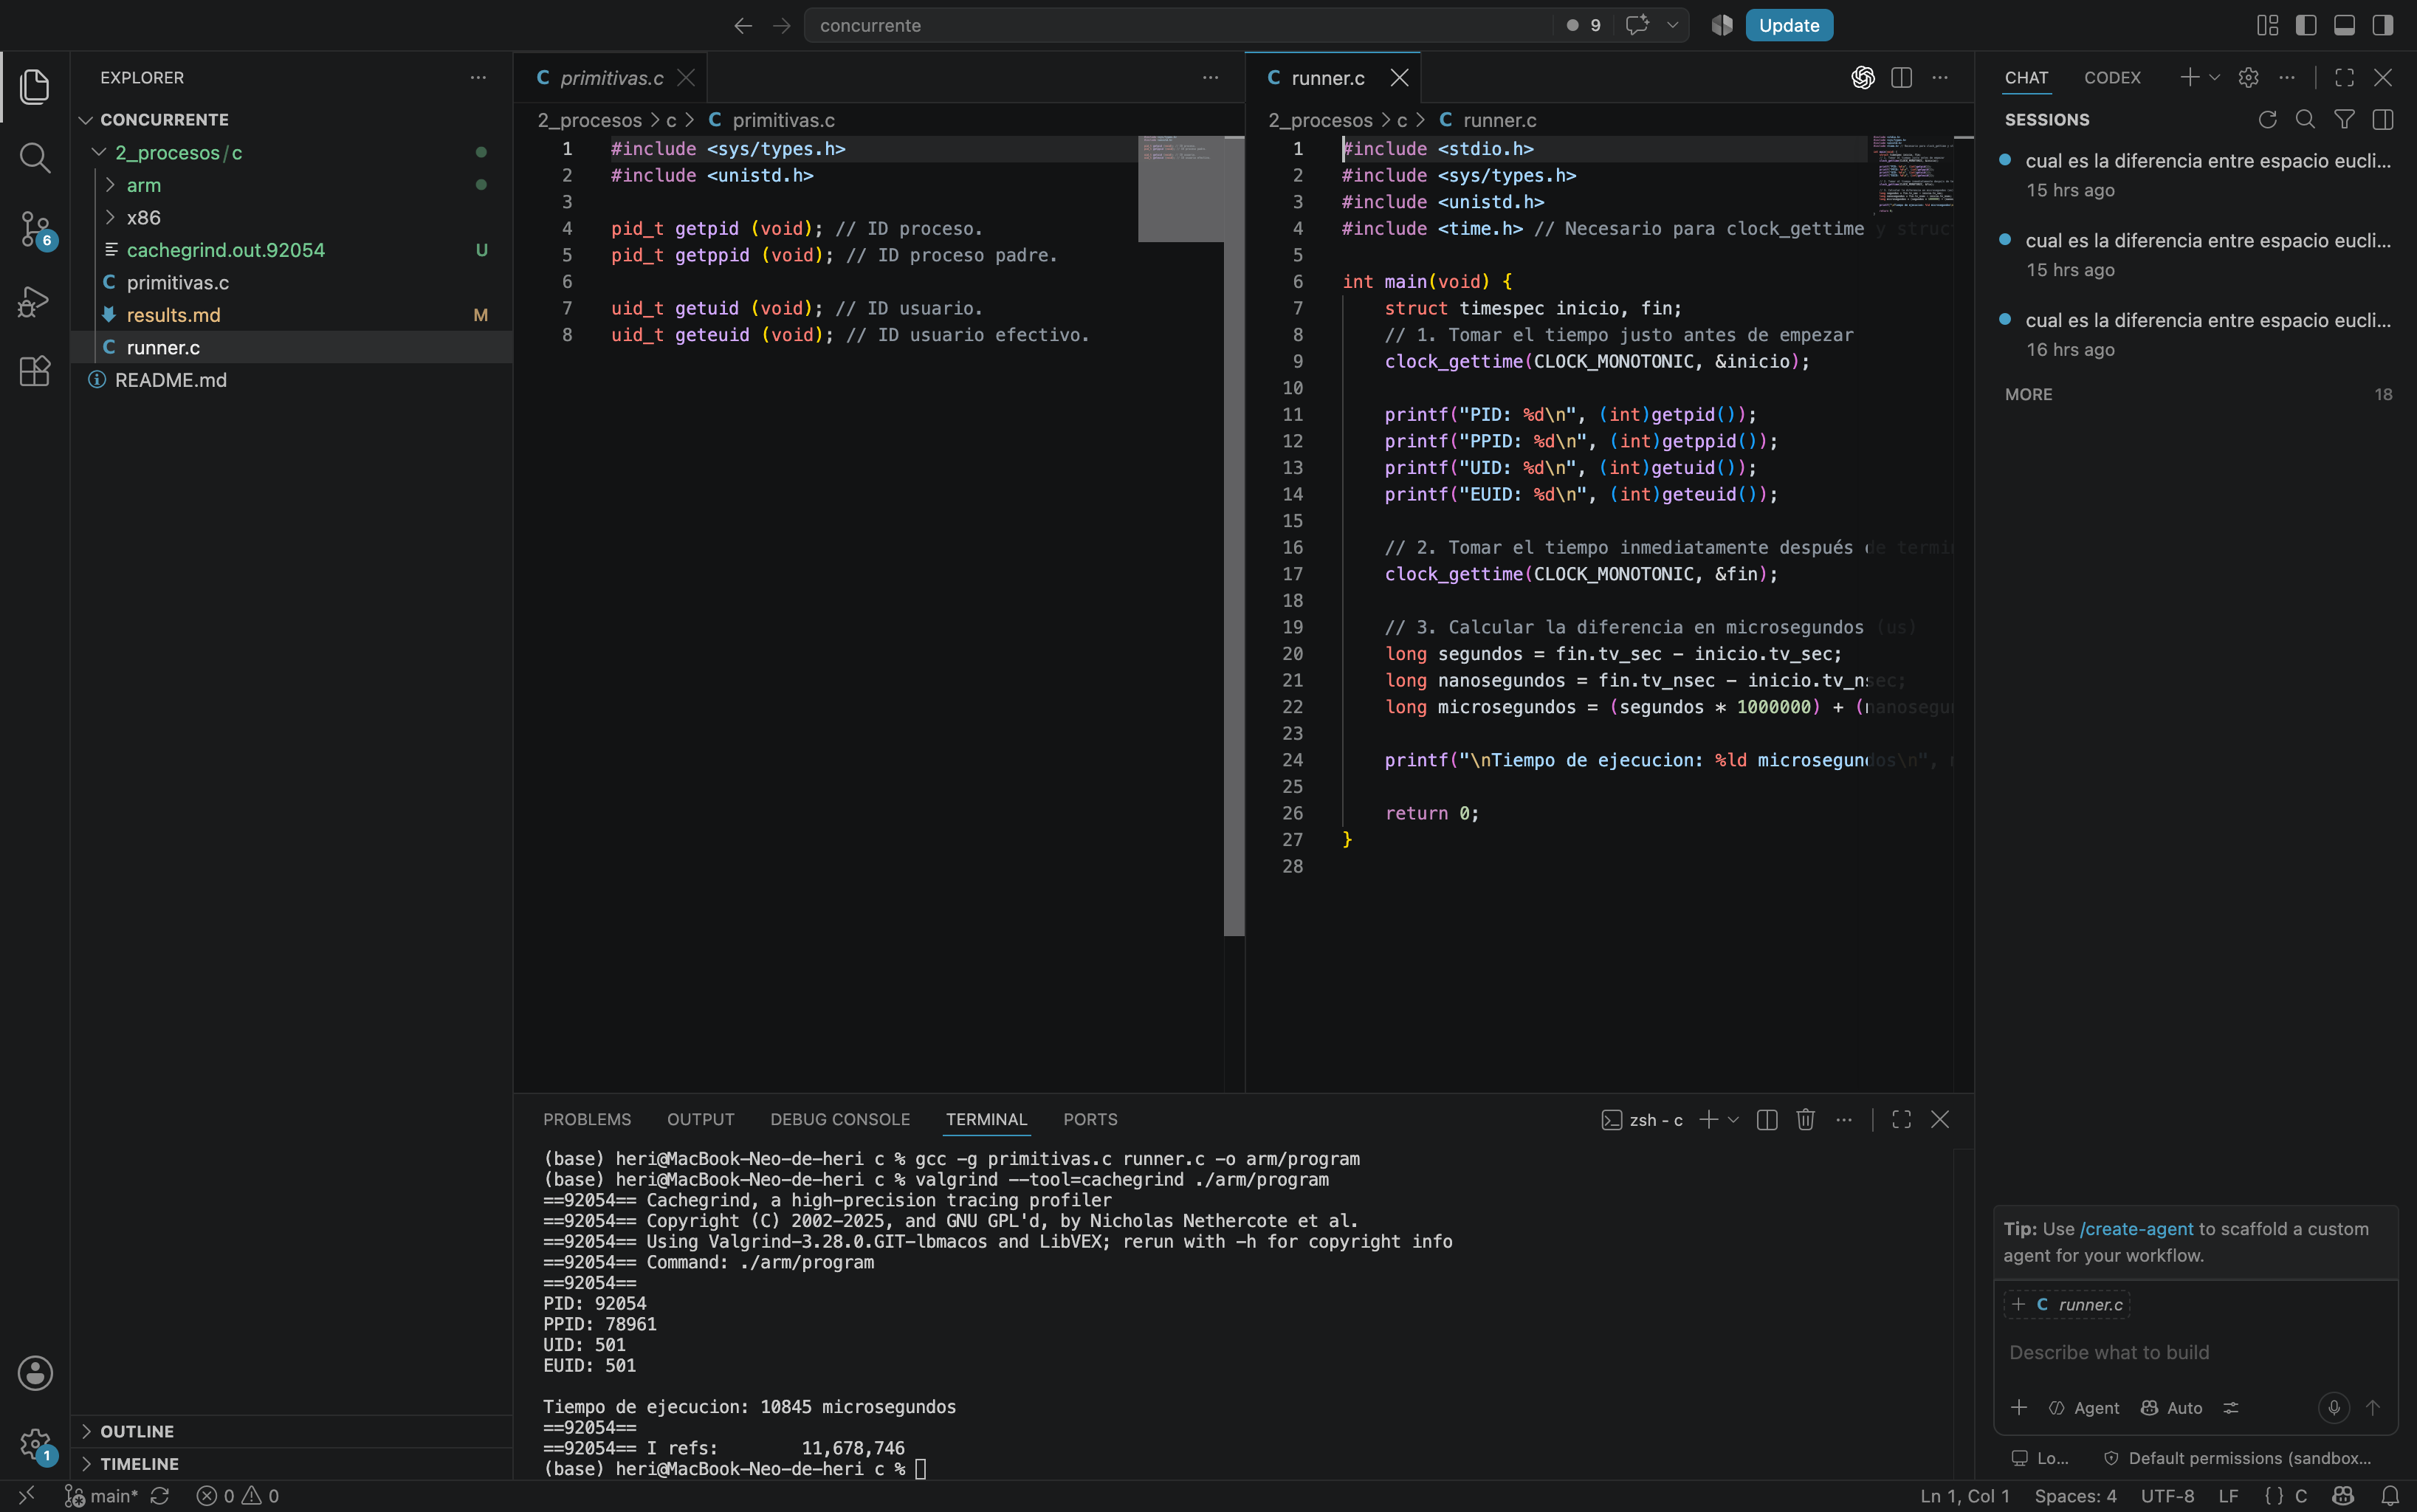
\includegraphics[width=0.73\textwidth]{5.png}
    \caption{Ejercicio 2 ejecutado en macOS en un procesador ARM}
    \label{fig:execution-macos}
\end{figure}

\section{Análisis Comparativo de Instrucciones e Identificadores: x86\_64 (WSL) vs. ARM64 (macOS)}

A partir de los reportes generados por la herramienta \texttt{Cachegrind} de Valgrind, se analiza la ejecución del programa C en dos arquitecturas de hardware distintas: un procesador Intel Core i5-13500H (x86\_64) corriendo bajo WSL (Linux) y un Apple A18 Pro (ARM64) corriendo en macOS nativo.

\subsection{Comparativa de Identificadores POSIX y Entornos de Ejecución}

Los metadatos extraídos por el programa reflejan las diferencias estructurales entre la capa de compatibilidad de Windows (WSL) y el sistema operativo macOS:

\begin{itemize}
    \item \textbf{Gestión de Usuarios (UID / EUID):} En el entorno WSL (Linux), el primer usuario no administrativo recibe por estándar el valor \texttt{1000} (\textbf{herie}). En macOS, la convención del sistema asigna el valor \texttt{501} a la cuenta del usuario principal (\textbf{heri}). En ambos escenarios, al no haber elevación de privilegios, $\text{UID} = \text{EUID}$.
    \item \textbf{Jerarquía de Procesos (PID / PPID):} En WSL, la terminal interactiva opera con el $\text{PPID} = 1326$, creando el proceso hijo con $\text{PID} = 39424$. En macOS, la terminal (\texttt{zsh}) bajo el proceso $\text{PPID} = 78961$ engendra al ejecutable asignándole el $\text{PID} = 92054$.
\end{itemize}


\subsection{Mapeo de Instrucciones (I refs) y Ecuación de Rendimiento de la CPU}

La métrica \textbf{I refs} (\textit{Instruction references}) representa el total de instrucciones procesadas. El tiempo total de ejecución depende de las características microarquitectónicas y a la frecuencia de reloj del procesador, aproximadamente:

$$T = \frac{IC \times CPI}{f}$$

Donde:
\begin{itemize}
    \item $T$: Tiempo de ejecución del procesador.
    \item $IC$ (\textit{Instruction Count}): Número total de instrucciones ejecutadas (\textbf{I refs}).
    \item $CPI$ (\textit{Cycles Per Instruction}): Promedio de ciclos de reloj requeridos para ejecutar una instrucción.
    \item $f$: Frecuencia de reloj del procesador (Hertz).
\end{itemize}

\subsection{Análisis Microarquitectónico: Intel i5-13500H vs. Apple A18 Pro}

Las discrepancias en los registros se explican por el diseño de cada chip:

\begin{itemize}
    \item \textbf{Intel Core i5-13500H (x86\_64 / CISC):} Este chip opera con una frecuencia máxima de $4.7\text{ GHz}$. CISC (\textit{Complex Instruction Set Computer}) permite codificar operaciones densas (como accesos a memoria y cálculos aritméticos) en una sola instrucción. Esto reduce el $IC$ ($140,811$ I refs), pero a costa de un $CPI$ más alto por instrucción.
    \item \textbf{Apple A18 Pro (ARM64 / RISC):} Opera con una frecuencia máxima de $4.04\text{ GHz}$ en sus núcleos de rendimiento. RISC (\textit{Reduced Instruction Set Computer}) usa operaciones sencillas. Esto genera un aumento de  $IC$ ($11,678,746$ I refs), compensada por un $CPI$ bajo (cercano a $1$ por ciclo). 
\end{itemize}

\chapter{Instrucciones e Identificadores en JAVA}

El código fuente anterior como lo implementaría en JAVA, agrega tu código en
JAVA y la captura de pantalla de su ejecución.

\begin{figure}[H]
    \centering
    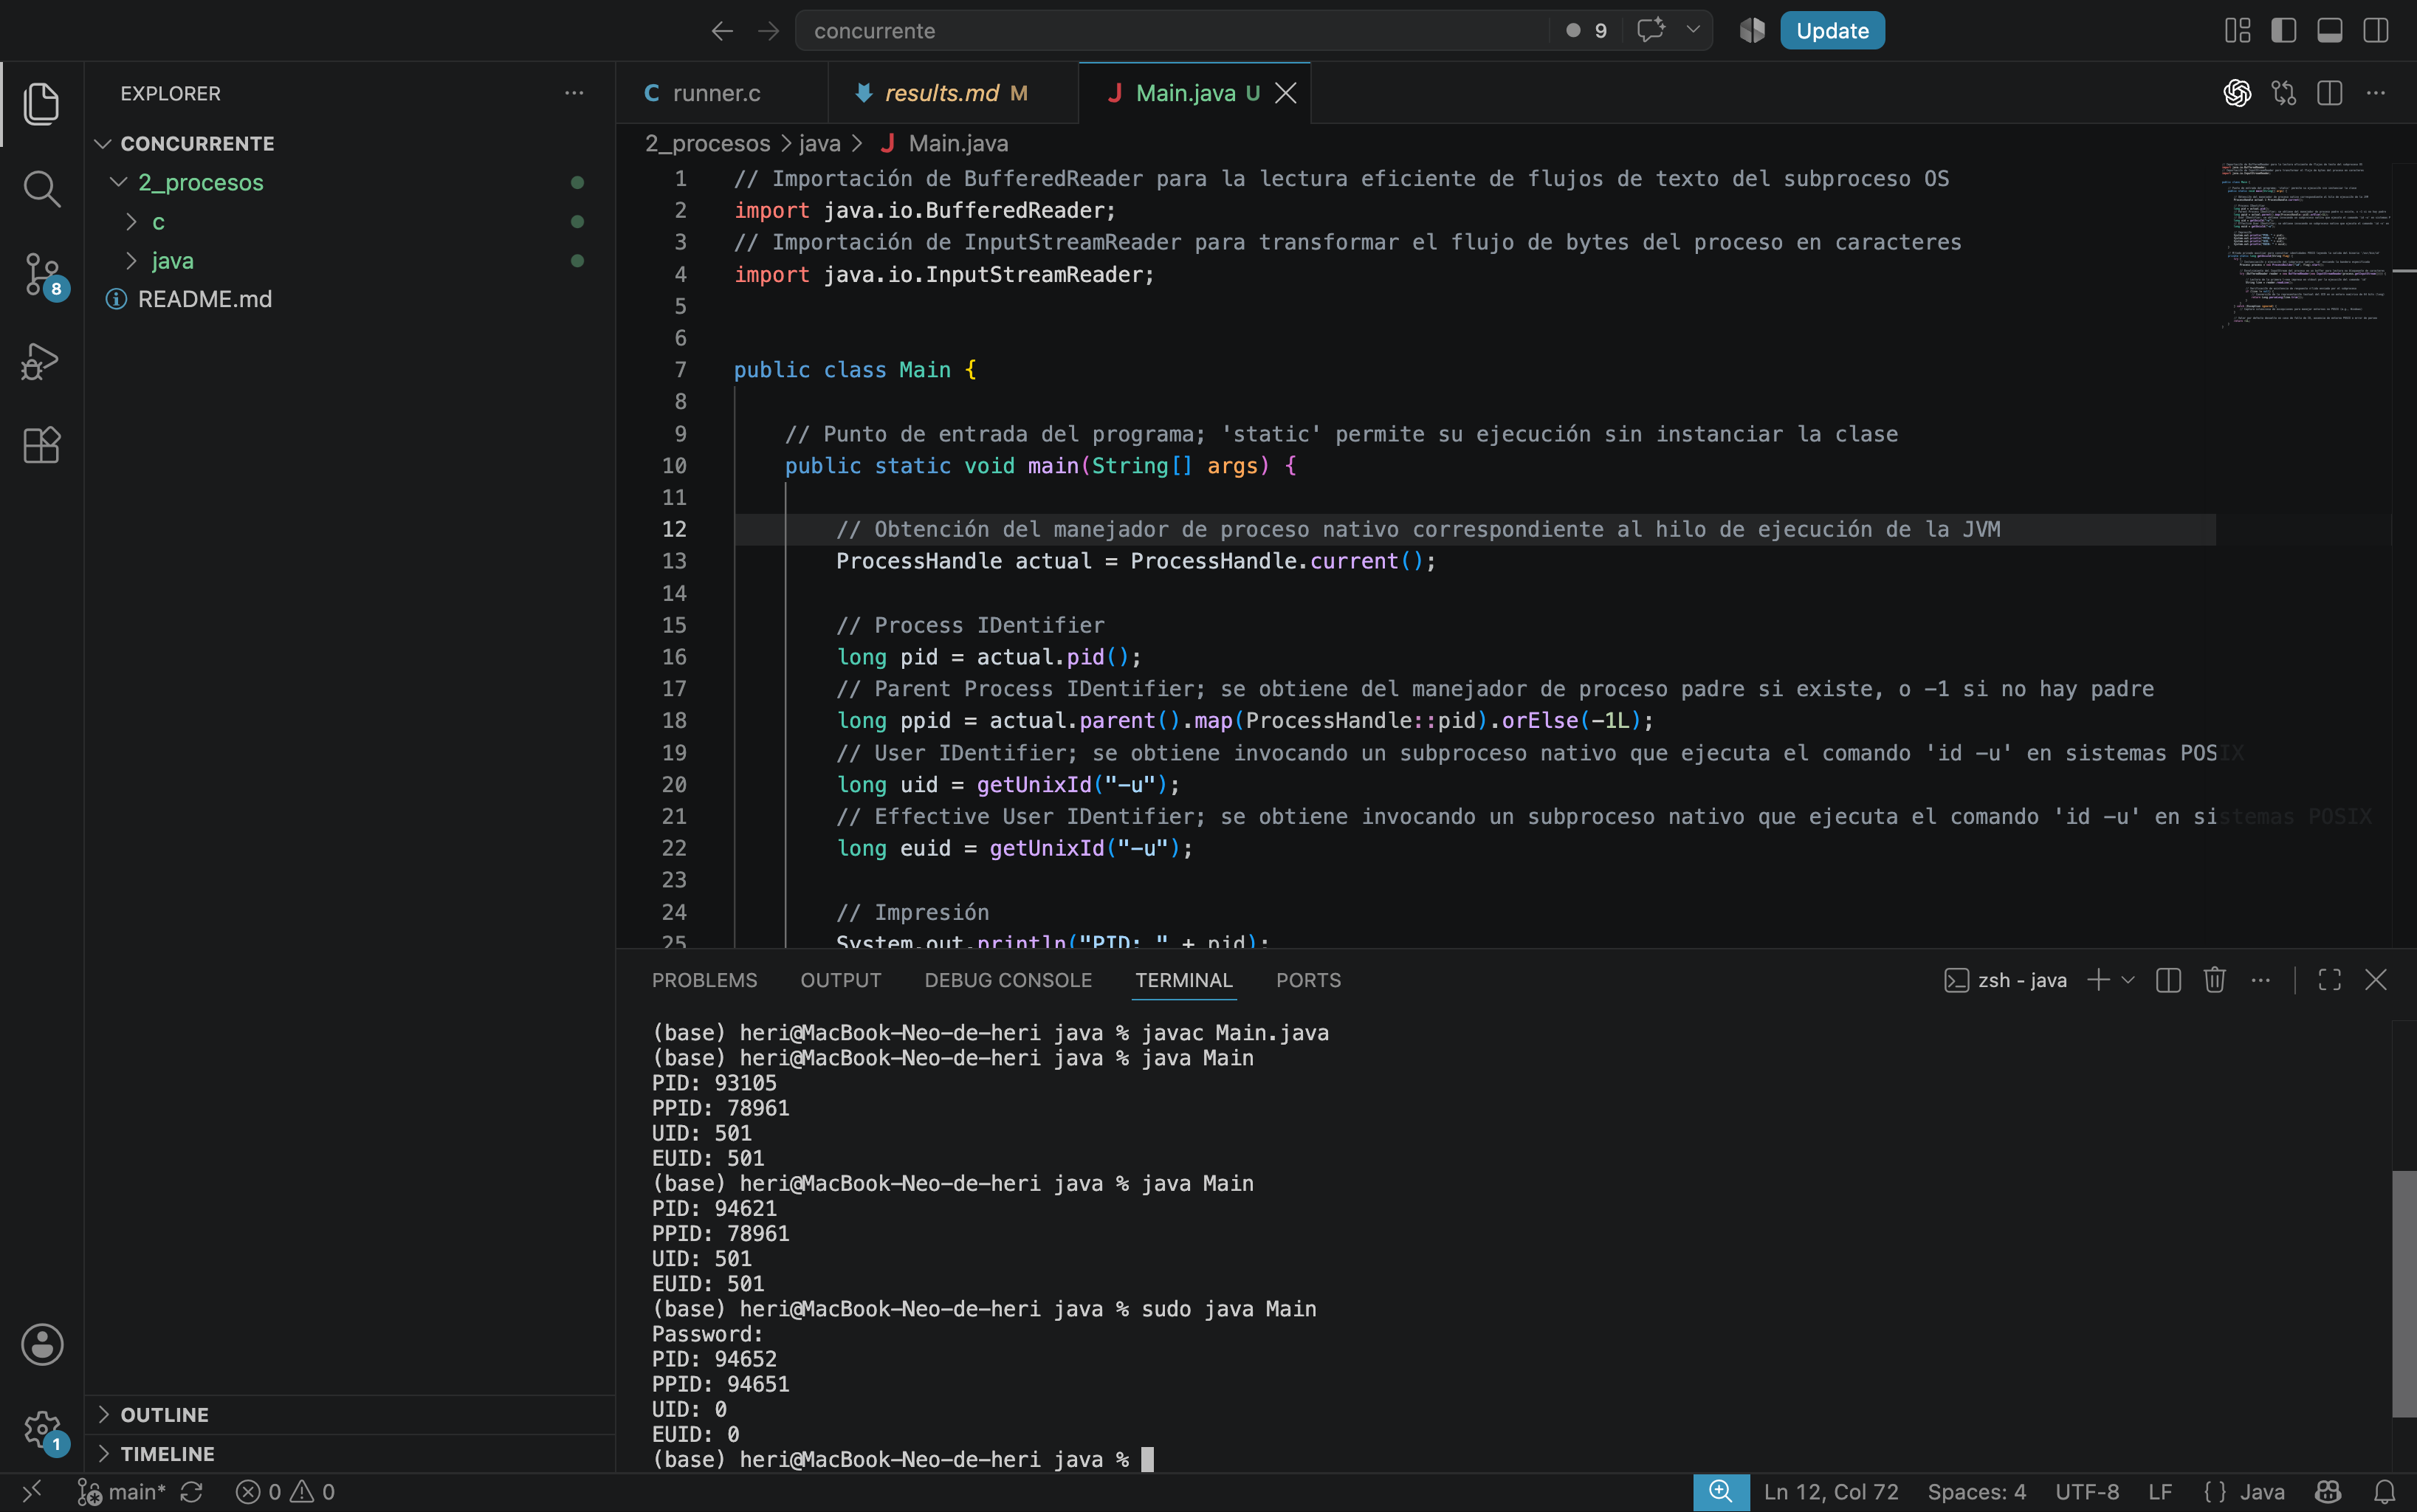
\includegraphics[width=0.73\textwidth]{6.png}
    \caption{Ejercicio ejecutado en JAVA}
    \label{fig:java-execution}
\end{figure}

\section{Análisis de Procesos}

Al ejecutar el programa desde la terminal de VS Code, el sistema operativo devuelve diferentes valores para los identificadores de proceso e identidad según el tipo de ejecución.

\subsection{Cambio de PID y Permanencia de PPID}

En las dos primeras ejecuciones (\texttt{java Main}), se observan los siguientes comportamientos:
\begin{itemize}
    \item \textbf{PID (\textit{Process ID}):} Cambia en cada ejecución (\texttt{93105} en la primera y \texttt{94621} en la segunda). Cada vez que se corre un programa, el sistema operativo le asigna un número de identificación único y temporal que se destruye al finalizar.
    \item \textbf{PPID (\textit{Parent Process ID}):} Se mantiene constante en \texttt{78961}. Esto ocurre porque ambas ejecuciones fueron lanzadas desde la misma ventana de la terminal (\texttt{zsh}). La terminal es el proceso "padre" que abre al programa "hijo". No se muestra en la figura, pero al abrir otra terminal se obtuvo \texttt{PPID: 94952}
\end{itemize}


\subsection{Cambio de Privilegios con \texttt{sudo} (UID y EUID)}

La tercera ejecución introduce el comando de elevación de permisos (\texttt{sudo java Main}):
\begin{itemize}
    \item \textbf{UID y EUID en ejecución normal:} En las primeras pruebas, ambos valores son \texttt{501}. En macOS, el número \texttt{501} es el identificador numérico asignado a la cuenta del primer usuario del sistema (\textbf{Heri}).
    \item \textbf{UID y EUID con \texttt{sudo}:} Al anteponer \texttt{sudo}, el sistema solicita la contraseña del usuario y cambia temporalmente la identidad de la ejecución. Tanto el \textbf{UID} como el \textbf{EUID} pasan a ser \texttt{0}, que es el identificador reservado para el administrador del sistema (\textit{root}).
    \item \textbf{Cambio de PPID:} El \textbf{PPID} cambia a \texttt{94651} porque el programa ya no es lanzado directamente por la terminal, sino por el proceso intermedio del comando \texttt{sudo}.
\end{itemize}

\cleardoublepage
\phantomsection
\addcontentsline{toc}{chapter}{Referencias}
\nocite{*} % El operador de revelación global; la negación del 
\bibliography{template/references}

\end{document}

